\documentclass{beamer}
\usepackage{amsmath}
\usepackage{tabularx}
\usepackage{graphicx}
\usepackage{tikz}
\usetikzlibrary{arrows.meta,automata,quotes,positioning,babel}
\usetikzlibrary{shapes.geometric, arrows}
\usepackage{hyperref}
\usepackage{float}

\title{Deep Learning Approach to Link Weight Prediction}
\author{Yuchen~Hou\inst{1} \and Lawrence~Holder\inst{1}}
\institute{
	\inst{1}
	School of Electrical Engineering and Computer Science\\
	Washington State University, Pullman, WA 99164
}

\begin{document}

\frame{\titlepage}

\begin{frame}{Introduction: deep learning in different domains}
%	\begin{itemize}[<+->]
	\begin{itemize}
		\item Image recognition
		\item Speech recognition
		\item Natural language processing
		\item Recommendation systems
		\item Graph mining (node, link and graph attributes)
	\end{itemize}
\end{frame}

\begin{frame}{Background: graph mining problems}
	\begin{table}[H]\centering
		\caption{
			Graph mining problems and examples in a few application domains.
		}
		\begin{tabularx}{\textwidth}{|X|X|X|}  \hline
			Problem & Problem example & Application domain \\ \hline
			Node classification & Alex is female & social network \\ \hline
			Node regression & Alex is 30 years old & social network \\ \hline
			Link prediction & Alex likes Bob & social network \\ \hline
			Link weight prediction & Alex texts Bob 128 times per day & social network \\ \hline
			Graph classification & Ethanol is toxic & chemical activity \\ \hline
			Graph regression & Ethanol has toxicity 0.53 & chemical activity \\ \hline
		\end{tabularx}
		\label{tab:problems}
	\end{table}
\end{frame}

\begin{frame}{Problem: link weight prediction}{Problem example}
	\begin{figure}[H]\centering
		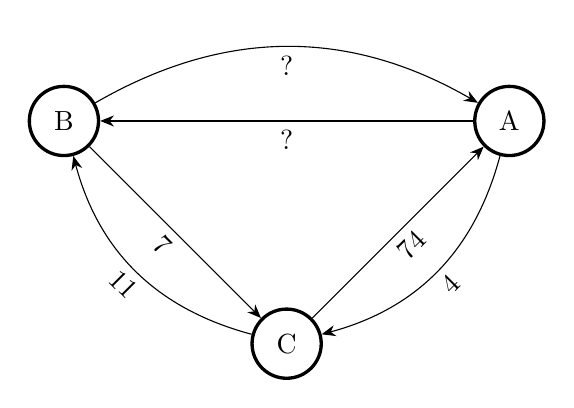
\begin{tikzpicture}[
		node distance = 4cm,
		on grid,
		> = {Stealth[length=5pt,width=4pt]},
		every state/.style = {very thick},
		every edge quotes/.style = {sloped, anchor=north}
		]
		\node[state] (B) {B};
		\node[state] (C) [below right=of B] {C};
		\node[state] (A) [above right=of C] {A};
		\path[->]   
		(A) edge["?"]   (B)
		(B) edge["7"]   (C)
		(C) edge["74"]  (A)
		(B) edge[bend left,"?"]   (A)
		(A) edge[bend left,"4"]   (C)
		(C) edge[bend left,"11"]  (B);
		\end{tikzpicture}
		\caption{
			An example of link weight prediction in a weighted directed graph -
			message volume prediction in a social network for friend recommendation.
		}
		\label{fig:example}
	\end{figure}
\end{frame}

\begin{frame}{Problem: link weight prediction}{Problem example}
	\begin{table}[H]\centering
		\caption{
			The same example but with edge list representation for the network.
		}
		\begin{tabularx}{\textwidth}{|X|X|X|}  \hline
			Source node & Destination node & Link weight \\ \hline
			A & B & ? \\ \hline
			A & C & 74 \\ \hline
			B & A & ? \\ \hline
			B & C & 7 \\ \hline
			C & A & 4 \\ \hline
			C & B & 11 \\ \hline
		\end{tabularx}
		\label{tab:example}
	\end{table}
\end{frame}

\begin{frame}{Problem: link weight prediction}{Problem definition}
	\begin{itemize}
		\item Given a weighted directed graph with the node set V and a link subset E
		\item Build a model w = f(x, y) to predict the weight w of any link (x, y) $ \notin $ E
	\end{itemize}
\end{frame}

\begin{frame}{Existing approach: SBM(Stochastic Block Model)}{Diagram illustration}
	Partition the graph into L groups so the graph has a 2-tier structure:
	\begin{itemize}
		\item Lower tier: each group consists of nodes which were topologically similar in the original graph
		\item Upper tier: groups are connected by bundles to represent the original graph
	\end{itemize}
	\begin{figure}[H]
		\centering
		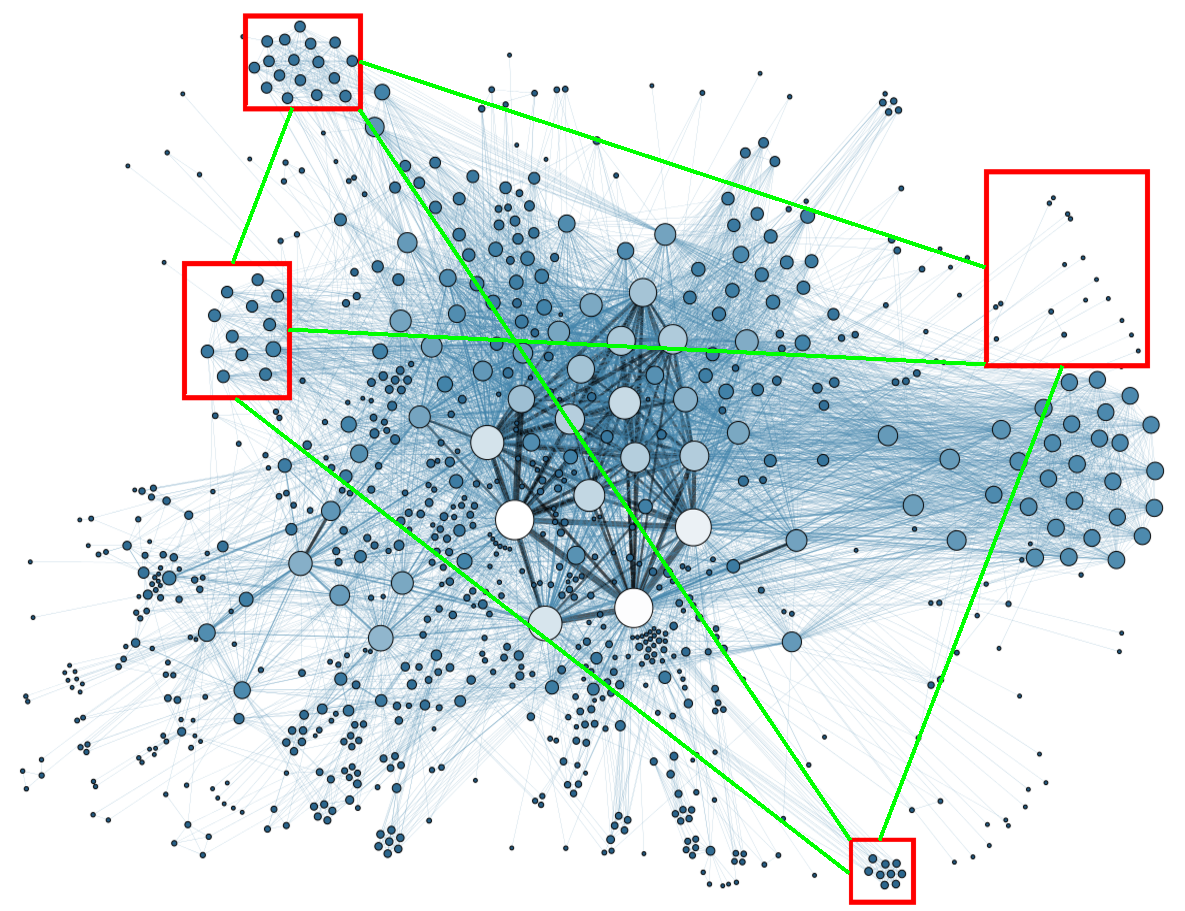
\includegraphics[width=0.4\linewidth]{SBM}
		\caption{ \href{https://commons.wikimedia.org/wiki/File:Social_Network_Analysis_Visualization.png}{Social Network Analysis Visualization}(Martin Grandjean / Wikimedia Commons / Attribution-Share Alike 3.0 Unported)}
		\label{fig:SBM}
	\end{figure}
\end{frame}

\begin{frame}{Existing approach: SBM(Stochastic Block Model)}{Formula illustration}
	Given a graph with adjacency matrix A, the SBM has the following parameters:
	\begin{itemize}
		\item $ z $: the group vector,
		where $ z_i \in \{ 1 ... L \} $ is the group label of node i
		\item $ (\mu, \sigma) $: the bundle weight distribution parameters,
		where $ (\mu_{z_i z_j}, \sigma_{z_i z_j}^2) $ is the weight distribution parameters of bundle ($z_i, z_j$)
	\end{itemize}
	The SBM models the weight of link (i, j) $ A_{ij} $ as a real random variable following the normal distribution:
	\begin{align*}
	A_{ij} \sim N(\mu_{z_i z_j}, \sigma_{z_i z_j}^2)
	\end{align*}
	The SBM fits parameters $ z $ and $ (\mu, \sigma) $
	to maximize the probability of observation A:
	\begin{align*}
	\log(P(A|z, \theta))
	&= \sum_{ij} (
	A_{ij} \frac{\mu_{z_i z_j}}{\sigma_{z_i z_j}^2}
	- A_{ij}^2 \frac{1}{2\sigma_{z_i z_j}^2}
	- \frac{\mu_{z_i z_j}^2}{\sigma_{z_i z_j}^2}
	)
	\end{align*}
\end{frame}

\begin{frame}{Deep learning approach: Model R}
	\begin{figure}[H]
		\centering
		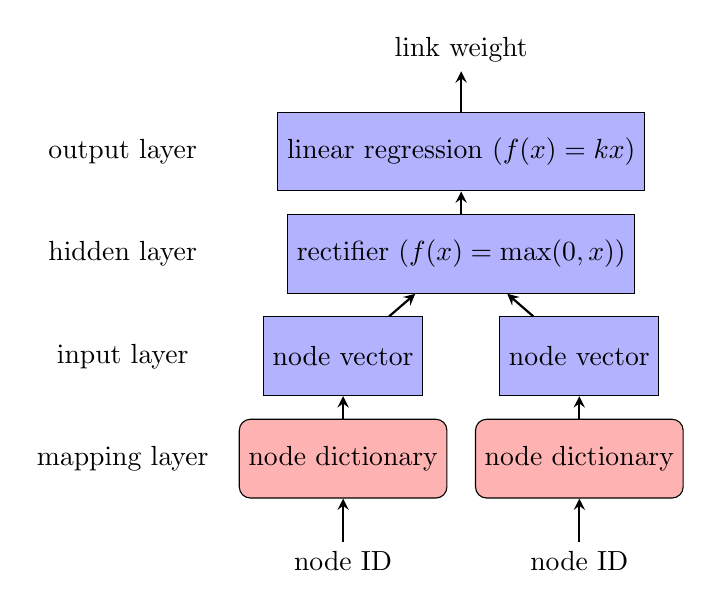
\begin{tikzpicture}[node distance=1.3cm]
		\tikzstyle{startstop} = [rectangle, rounded corners, minimum width=1cm, 
		minimum height=1cm, text centered, draw=black, fill=red!30]
		\tikzstyle{process} = [rectangle, minimum width=1cm, minimum height=1cm, 
		text centered, draw=black, fill=blue!30]
		\tikzstyle{arrow} = [thick,->,>=stealth]
		\node (linearRegression) [process] {linear regression ($ f(x) = kx $)};
		\node (relu) [process, below of=linearRegression] {rectifier ($ f(x) = \max (0, x) $)};
		\node (linear1) [process, below of=relu, xshift=-1.5cm] {node vector};
		\node (linear2) [process, below of=relu, xshift=1.5cm] {node vector};
		\node (oneHot1) [startstop, below of=linear1] {node dictionary};
		\node (oneHot2) [startstop, below of=linear2] {node dictionary};
		\node (weight) [above of=linearRegression] {link weight};
		\node (output) [left of=linearRegression, xshift=-3cm] {output layer};
		\node (hidden) [below of=output] {hidden layer};
		\node (input) [below of=hidden] {input layer};
		\node (mapping) [below of=input] {mapping layer};
		\node (source) [below of=oneHot1] {node ID};
		\node (destination) [below of=oneHot2] {node ID};
		\draw [arrow] (source) -- (oneHot1);
		\draw [arrow] (destination) -- (oneHot2);
		\draw [arrow] (oneHot1) -- (linear1);
		\draw [arrow] (oneHot2) -- (linear2);
		\draw [arrow] (linear1) -- (relu);
		\draw [arrow] (linear2) -- (relu);
		\draw [arrow] (relu) -- (linearRegression);
		\draw [arrow] (linearRegression) -- (weight);
		\end{tikzpicture}
		\caption{
			The Model R (R as in "relation") for graph weight link prediction.
		}
		\label{fig:model}
	\end{figure}
\end{frame}

\begin{frame}{Experiments}{Datasets}
	\begin{table}[H]\centering
		\caption{The datasets used in experiments.}
		\begin{tabularx}{\textwidth}{|X|X|X|}  \hline
			Dataset & Node count & Link count \\ \hline
			Airport & 500 & 5960 \\ \hline
			Collaboration & 226 & 20616 \\ \hline
			Congress & 163  & 26569 \\ \hline
			Forum  & 1899 & 20291 \\ \hline
		\end{tabularx}
		\label{tab:datasets}
	\end{table}
\end{frame}

\begin{frame}{Experiments}{Results}
	\begin{figure}[H]\centering
		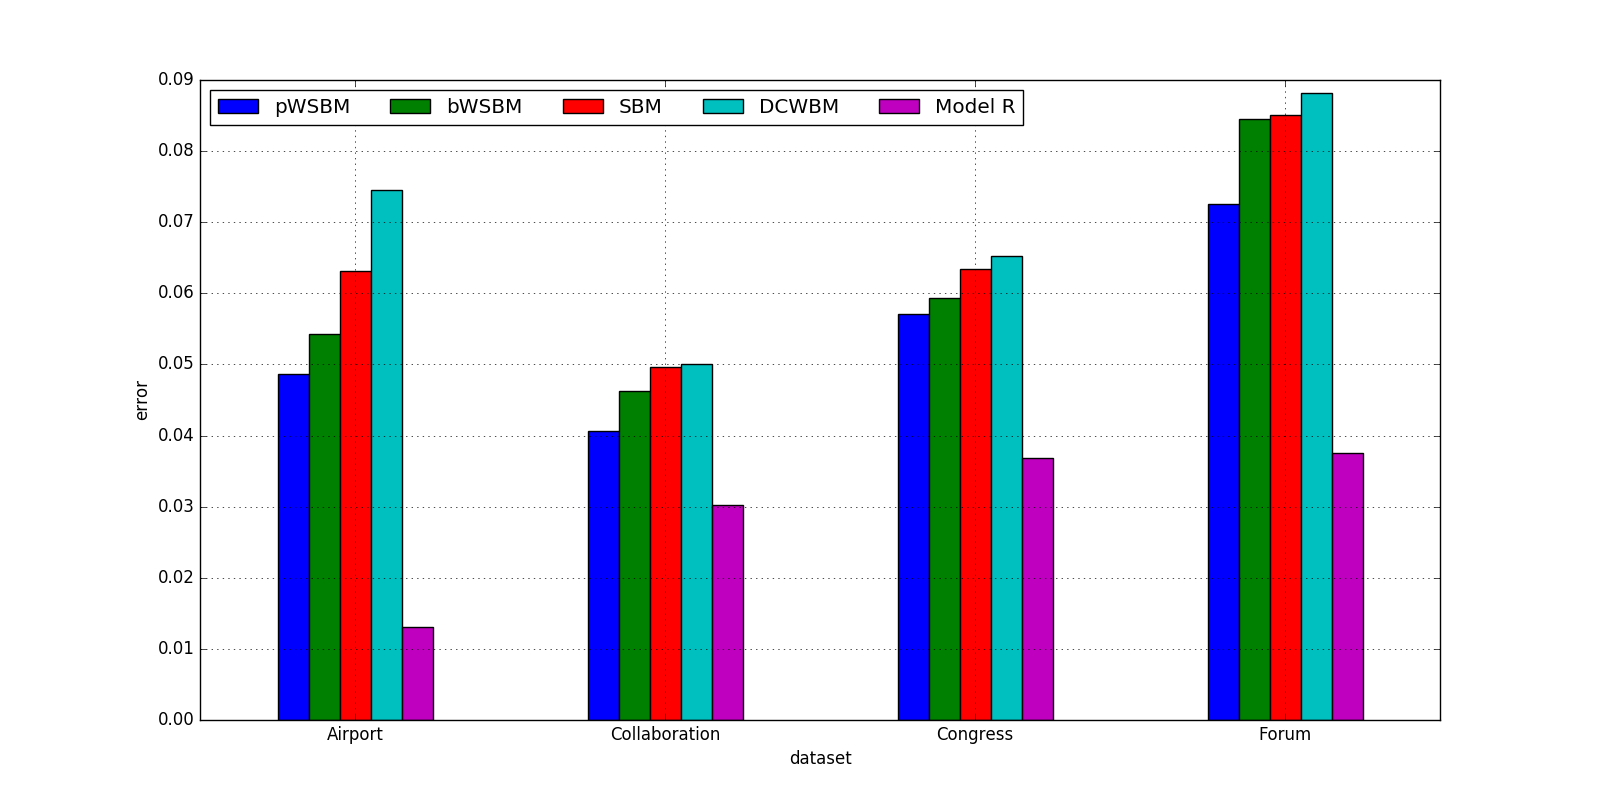
\includegraphics[width=\textwidth]{link-weight-errors}
		\caption{
			The mean squared errors of 5 models (SBM and its 4 derivatives pure weighted SBM, balanced weighted SBM, degree corrected weighted SBM, Model R) on 4 datasets:
			Model R has the lowest error consistently.
		}
		\label{fig:errors}
	\end{figure}
\end{frame}

\begin{frame}{Conclusions}
	\begin{itemize}
		\item Model R learns node information (i.e., node vectors) from node relations (i.e., link weight)
		\item Model R uses node vectors to predict unknown link weights.
		\item Model R is more accurate than Stochastic Block Model based approaches
		\item Deep learning can be successfully applied to link weight prediction problem
	\end{itemize}
\end{frame}

\end{document}